\documentclass[8pt]{article}
% Эта строка — комментарий, она не будет показана в выходном файле
\usepackage{ucs}
\usepackage[utf8x]{inputenc} % Включаем поддержку UTF8
\usepackage[russian]{babel}  % Включаем пакет для поддержки русского языка
\usepackage{amsmath}
\usepackage{mathtools}
\usepackage{amssymb}
% \usepackage[dvips]{graphicx}
% \graphicspath{{noiseimages/}}
\usepackage[pdftex]{graphicx}


% Параметры страницы: 1см от правого края и 2см от остальных.


\hoffset=0mm
\voffset=0mm
\textwidth=180mm        % ширина текста
\oddsidemargin=-6.5mm   % левое поле 25.4 - 5.4 = 20 мм
\textheight=240mm       % высота текста 297 (A4) - 40
\topmargin=-15.4mm      % верхнее поле (10мм)
\headheight=5mm      % место для колонтитула
\headsep=5mm          % отступ после колонтитула
\footskip=8mm         % отступ до нижнего колонтитула


\begin{document}
    \author {Зотов Алексей 496 гр.}
    \title {Лабораторная работа 1.5 \\  Изучение колебаний струны}
    \maketitle{}   

    \textbf{Цель работы:} изучение поперечных стоячих волн в струне: определение собственных частот колебания струны в зависимости от натяжения струны и определение скорости распространения поперечных волн в струне. 

    Ограниченная, закрепленная на концах струна, может совершать собственные колебания, представляющие собой стоячие волны вида:
    \begin{equation}
        y(x,t) = A\sin \left (2 \pi f t \right )\sin \left(\frac{2\pi}{\lambda}x \right)
    \end{equation}

    где $A$— амплитуда колебаний в пучностях, $f$ — частота, $\lambda$ — длина волны, $x$ — координата вдоль струны. В концевых точках должны располагаться узлы стоячей волны (амплитуда колебаний равна нулю), откуда следует, что на струне длиной $L$ должно укладываться целое число полуволн:
    \begin{equation}
        L = n \frac{\lambda_n}{2}, \quad n = 1,2,3\dots        
    \end{equation}

    Скорость распространения поперечных волн $u$ зависит от силы натяжения струны $F$ и массы струны на единицу длины 
    $\rho _l$ погонной плотности струны $\rho _l  = \rho S$):
    \begin{equation}
        u = \sqrt{\frac{F}{\rho_l}}
    \end{equation}

    Возможные частоты собственных колебаний струны (обертоны):
    \begin{equation}
        f_n = \frac{u}{\lambda_n} = \frac{n}{2L}\sqrt{\frac{F}{\rho_l}} 
    \end{equation}

    Если частота внешней поперечной синусоидальной силы совпадает с какой либо собственной частотой колебания струны, то возникает явление резонанса и образуется синусоидальная стоячая волна.

    \textbf{В работе используются:} звуковои генератор, двухканальный осциллограф, частотомер, набор грузов, станина, с закрепленной на ней струной (Рис.1).

    \begin{center} 
        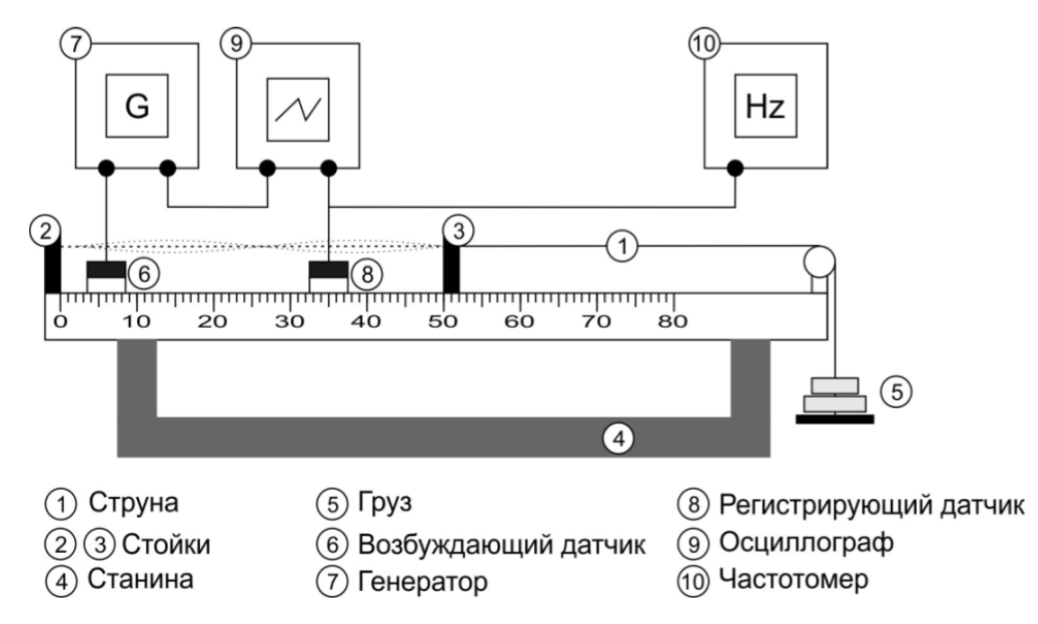
\includegraphics[width=3.5in]{string_img.png} \\ Рис. 1: Экспериментальная установка.
    \end{center}
    
    \textbf{Ход работы:}\\
    
\end{document}